%!TEX root = thesis.tex

%overview of the methodology to be used;

\chapter{Methods}
\label{chap:methods}

A number of studies related to this thesis have been reviewed in Chapter \ref{chap:rw}. This chapter discusses why the semantic web will be used for linking sensor metadata and which methods will be used to achieve this. The \ac{swe} standards, the om-lite and sam-lite ontologies, and \ac{rdf} will be described.  

\section{Sensor metadata on the semantic web}
\ac{semsos} \citep{SSW:Henson, SSW:Pschorr} as well as \ac{sel} \citep{SSW:Janowicz} focus on combining the sensor web with the semantic web, but do not address the integration and aggregation of sensor data. Similarly, \cite{SSW:Atkinson} proposes to expose sensor data to the semantic web in order to find other kinds of related data about the same feature-of-interest. Data that can be collected for another area of research. However, \cite{SSW:Atkinson} do not mention the integration of complementary sensor data from heterogeneous sources either. \cite{SSW:Stasch} and \cite{SSW:Stasch3} suggest interesting methods for aggregating sensor data based on features-of-interest. However, also these studies use sensor data from only a single source into account. Moreover, \cite{SSW:Corcho} and \cite{SSW:Ji} argue that methods for integration and fusion of sensor data on the semantic web is still an area for future research. Data fusion is \enquote{a data processing technique that associates, combines, aggregates, and integrates data from different sources} \cite[p. 2]{SSW:Wang2}. 

\cite{SW:OGC3} and \cite{SW:OGC4} present methods for including \ac{sos} services in an \ac{ogc} catalogue service using \ac{sor} and \ac{sir}. Making sensor metadata available in a catalogue service will improve the discovery. However, discovery through the semantic web is likely to be more effective, since links can be created towards the sensor data from many different sources of related information. Another advantage is that links can be created by everybody that publishes linked data on the web, allowing sensor data to be used for implementations that were not identified beforehand by the publisher. Also, the semantic web will be easier to access, while the catalogue service can only be requested at a certain \ac{url} which has to be known to potential users. 

Since data on the web has a distributed nature it can be questioned whether centralised catalogue services are feasible to create. It places a burden on the owner of the \ac{sos} to register with a catalogue service. Also, there could be multiple of these services on the web creating issue regarding the discovery of relevant catalogues. The semantic web could solve this issue by getting rid of the `dataset-centric' approach and adding metadata directly to the web instead.

\section{Sensor observation service}
There are a number of different requests that can be made to retrieve sensor (meta)data from a \ac{sos}: \texttt{GetCapabilities, DescribeSensor and GetObservation}. \texttt{GetCapabilities} returns a complete overview of what the \ac{sos} has to offer. This includes metadata on the kind of observations the service can offer, the spatial extent and the temporal extent. The  \texttt{DescribeSensor} request returns detailed information about individual sensors. Using \texttt{GetObservation} actual measurements can be retrieved. These requests can be made as a \ac{http} GET request or a \ac{http} POST request. The response is an \ac{xml} document using \ac{om} (for GetObservation) or \ac{sensorml} (for DescribeSensor).

\section{Resource description framework}
For publishing static geographic data on the semantic web a conversion of Shapefiles to \ac{rdf} is required. For this the method by \cite{LD:Missier} will be used. First the Shapefile is loaded into a Postgres database with the Postgis extension. After that a Python script retrieves the records from the database. Attributes of the records will be mapped to classes from predefined ontologies. Then the script creates an \ac{rdf} graph and serialises it to a certain \ac{rdf} notation. This is written to a file. The final step is to publish the \ac{rdf} on the web and create a \ac{sparql} endpoint to query the data \citep{LD:Missier}. 

In \ac{rdf} data is stored as so-called `triples'. These triples are structured as: subject, predicate and object \citep{LD:Berners-lee}. The subject and the object are things and the predicate is the relation between these two things. For example, to define a geographic feature such as the municipality of Delft on the semantic web a number of triples can be made. Figure \ref{fig:Triples} shows how Delft can be defined as a municipality with a certain geometry using triples of subject, predicate and object.

\begin{figure}
	%\centering
	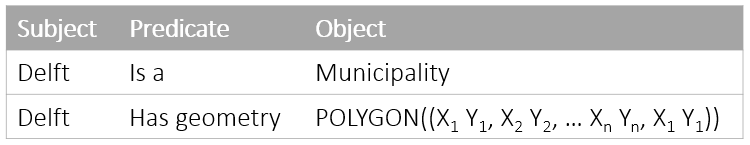
\includegraphics[width=0.7\linewidth]{figs/Triples.png}
	\caption{Triples of object, predicate and subject define Delft as a municipality with a geometry}
	\label{fig:Triples}
\end{figure}

Three types of data can make up these triples. The first type is an \ac{iri}. This is a reference to a resource and can be used for all positions of the triple. A \ac{url} is an example of an \ac{iri}, but \ac{iri}s can also refer to resources without stating a location or how it can be accessed. An \ac{iri} is a generalisation of an \ac{uri}, and also allows non-ASCII characters. In the example of the municipality of Delft, \ac{iri}s can be used to define `Delft' and `Municipality', but also for the predicates `is a' and `has geometry'. The second type of data is a literal. A literal is a value which is not an \ac{iri}, such as strings, numbers or dates. These values can only be used as object in a triple. In the example of Delft, a literal could be used to store the actual geometry of the boundary: POLYGON($x_{1},y_{1}$ $x_{2},y_{2}$ ... $x_{n},y_{n}$). Sometimes it is useful to refer to things without assigning them with a global identifier. The third type is the blank node and can be used as an subject or object without using an \ac{iri} or literal \citep{LD:W3C6}.  

There are a number of different notations for writing down these triples (serialisation), such as \ac{xml} \citep{LD:W3C3}, N3 \citep{LD:W3C5} and Turtle \citep{LD:W3C4}. Turtle will be used in this thesis, because it is is used for the object `Municipality'. The `is a' predicate is represented by a built-in \ac{rdf} predicate which can be written simple as `a'. The second predicate is `hasGeometry' for which the GeoSPARQL \ac{iri} is used. The geometry is a literal in the \ac{wkt} format. Note that the subject is only written once when there are multiple triples with the same subject. Triples that shares the same subject are divided by semicolons. A point marks the end of the last triple with a specific subject.

\begin{figure}
	%\centering
	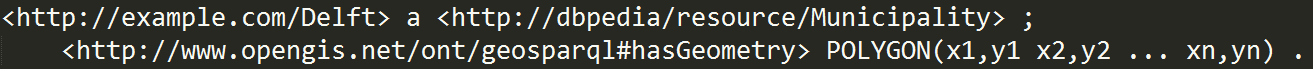
\includegraphics[width=1\linewidth]{figs/Turtle.png}
	\caption{Triples of Figure \ref{fig:Triples} in the Turtle notation}
	\label{fig:Turtle}
\end{figure}

The sensor metadata will also be published on the semantic web. To do this an \ac{xml} document is automatically retrieved from a \ac{sos} by a Python script. This script then extracts the relevant data from the \ac{xml} and maps it to an ontology. It outputs an \ac{rdf} file that will be published online. When new sources of sensor data are added the \ac{rdf} documents will be updated.   

\section{Ontology mapping}
When publishing data on the semantic web, ontologies are required to specify what things are and how they relate to other things. The evaluation of observation metadata ontologies by \cite{SW:Hu} is interesting, since it exposes what the relevant aspects are in the process of observation discovery. However, their proposed model focusses mainly on including remote sensing and imagery data in metadata models that were not originally created for this kind of data. The \ac{ssno} is an ontology that clearly describes the process between sensor, stimulus and observation. However, \cite{SSW:Cox4} points out that an important aspect of describing a sensor network is missing in this ontology: the sampling. Also, the om-lite and sam-lite ontologies by \cite{SSW:Cox4} are lightweight ontologies that can be complemented by already existing linked data ontologies. They do not rely on the (heavy) \ac{iso} specifications that date from before the semantic web, unlike the \ac{ssno}. The om-lite and sam-lite ontologies will therefore be used in this thesis. 

The \ac{uml} diagram (Figure \ref{fig:UML}) describes different components of a \ac{sos}. The \ac{sos} has a number of metadata attributes such as the service provider's details (including contact information), its spatial and temporal extent (spatialFiler \& temporalFilter) and the capabilities to query a subset of this extent. It receives data from a sensor which makes observations. An observation can be defined as \enquote{an action whose result is an estimate of the value of some property of the feature-of-interest, obtained using a specified procedure} \citep{SSW:Cox3}.The sensor is placed at a sampling point. The sampling point is part of a sampling feature which intents to resemble the feature-of-interest. In the case of air quality the feature-of-interest is the bubble of air surrounding the sensor, therefore the sampling point equals the feature-of-interest \citep{SDI:INSPIRE2}. The design is that an observation of the sampling feature describes the  feature-of-interest through measuring one of its properties. The measurement procedure is described by a short string of text, input and output parameters and the units of measurement of the ouput. The relation between feature-of-interest and administrative units is added to improve the discovery of sensor data on the semantic web. 

To publish data on the semantic web ontologies are required to specify the different classes and their relations. An ontology for static geographic data has to be connected to an ontology for sensor metadata. From the \ac{uml} diagram in Figure \ref{fig:UML} the classes Observation, Process, ObservedProperty and FeatureOfInterest can be mapped to classes belonging to \ac{owl} for observations \citep{SSW:Cox}. SamplingFeature and Sampling point can be mapped to classes from \ac{owl} for sampling features \citep{SSW:Cox2}. GeoSPARQL can be used for the administrativeUnit class \citep{LD:OGC} and the PROV ontology for the sensor and sensor observation service classes \citep{LD:W3C2}. 

\begin{figure}
	\centering
	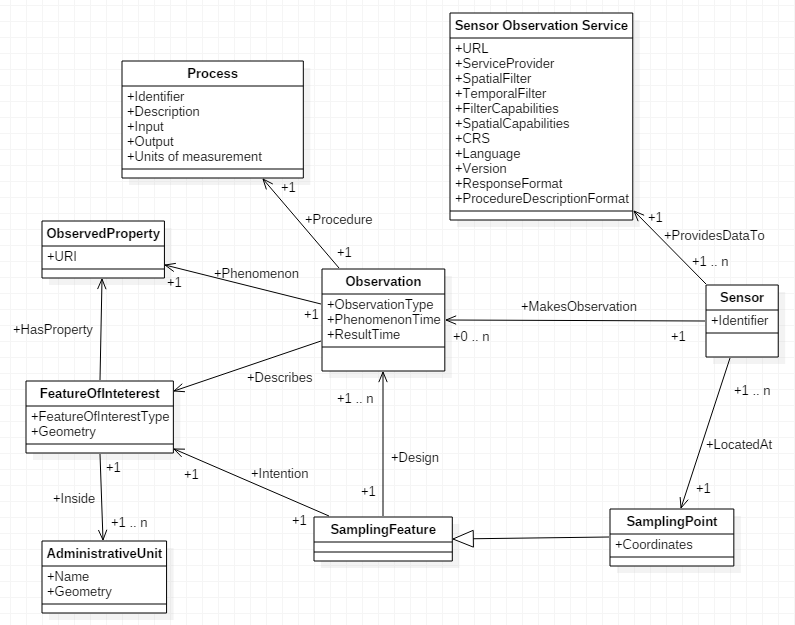
\includegraphics[width=1\linewidth]{UML/UML_Diagram.png}
	\caption{\ac{uml} diagram of sensor observations service, based on \cite{SSW:Cox3} and \cite{SDI:INSPIRE2}}
	\label{fig:UML}
\end{figure}

\section{Sensor data aggregation}
There are many different ways to aggregate sensor data, for example by taking the minimum value, the maximum value, the average value, the sum, etc. Also, spatial aggregation techniques (based on neighbourhood analysis) can be considered to adjust for spatio-temporal irregularities as mentioned by \cite{SW:Ganesan}. In order to determine which method of aggregation is applicable for a specific kind of sensor data the sensor metadata will contain links to appropriate aggregation methods. However, which methods are appropriate should be based on expert knowledge.

